\section{Generalisation Enhancement through PAC Bayesian Theory}\label{chap:generalisationPAC}


Since the invention of the PAC-Bayesian framework~\cite{mcallester1999pac}, there have been a number of canonical works developed in the past decades, including the parametrisation of the PAC-Bayesian bound with Gaussian distribution~\cite{langford2002not,langford2003pac}, the early works about generalisation error bounds for learning problems~\cite{germain2009pac,maurer2004note,parrado2012pac,welling2011bayesian} and the recent works about PAC-Bayes for machine learning models~\cite{alquier2016properties,blundell2015weight,dwork2015generalization,dwork2015preserving,dziugaite2018data,letarte2019dichotomize,perez2021tighter,rivasplata2019pac,thiemann2017strongly}. In the following, we will present a novelty method to improve DNN's generalisation performance through PAC-Bayesian theory.   


Given a prior distribution over the parameter $\theta$, which is selected before seeing a training dataset, a posterior distribution on $\theta$ will depend on both, the training dataset and a specific learning algorithm. The PAC-Bayesian framework~\cite{mcallester1999pac} bounds the generalisation error with respect to the KL divergence~\cite{KL1951} between the posterior and the prior distributions.


Consider a training dataset $D_{train}$ with $m \in \mathbb{N}$ samples drawn from a distribution $\mathcal{D}$. Given a learning algorithm (e.g., a classifier) $f_\theta$ with prior and posterior distributions $P$ and $Q$ on the parameter $\theta$ respectively, 
for any $\delta > 0$,
with probability $1-\delta$ over the draw of training data, we have that~\cite{dziugaite2017computing,mcallester1999pac} 
\begin{equation}
\label{eq:pac}
\mathbb{E}_{\theta \sim Q}[\mathcal{L}_\mathcal{D}(f_\theta)]\le \mathbb{E}_{\theta \sim Q}[\mathcal{L}_{D_{train}}(f_\theta)] + \sqrt{\frac{\mathrm{KL}(Q || P)+\log \frac{m}{\delta}}{2(m-1)}},
\end{equation}
where $\mathbb{E}_{\theta \sim Q}[\mathcal{L}_\mathcal{D}(f_\theta)]$ is the expected loss on $\mathcal{D}$, $\mathbb{E}_{\theta \sim Q}[\mathcal{L}_{D_{train}}(f_\theta)]$ is the empirical loss on $D_{train}$, and their difference yields the generalisation error. Equation~\ref{eq:pac} outlines the role KL divergence plays in the upper bound of the generalisation error. In particular, a smaller KL term will help tighten the generalisation error bound.  
Assume that $P$ and $Q$ are Gaussian distributions with $P=\mathcal{N}(\mu_P,\Sigma_P)$ and $Q=\mathcal{N}(\mu_Q,\Sigma_Q)$, then the
$\mathrm{KL}$-term can be written as follows:
\begin{equation}
\label{formula4}
\begin{aligned}
    &\mathrm{KL}(\mathcal{N}(\mu_Q,\Sigma_Q)||\mathcal{N}(\mu_P,\Sigma_P))\\
    &=\frac{1}{2}\Big[ \mathrm{tr}(\Sigma_P^{-1} \Sigma_Q)+(\mu_Q-\mu_P)^\top \Sigma_P^{-1}(\mu_Q-\mu_P)-k+\ln{\frac{\mathrm{det}\Sigma_P}{\mathrm{det}\Sigma_Q}} \Big],
\end{aligned}
\end{equation}
where $k$ is the number of parameters in $\theta$. Below, \cite{jin2020does}  incorporates weight correlation into this framework to tighten the bound. 


\subsection*{Weight Correlation in Fully Connected Neural Network (FCN).} Given weight matrix $w_l \in \mathbb{R}^{N_{l-1} \times N_l}$ of the $l$-th layer ($N_l$ is the number of neurons of the $l$-th layer), the average weight correlation of FCN is defined as
\begin{equation}
    \rho(N_l) =\frac{1}{N_l(N_l-1)} \sum_{i,j=1 \atop i \ne j}^{N_l} \frac{|w_{l i}^T w_{l j}|}{||w_{l i}||_2 ||w_{l j}||_2},
\end{equation}
where $w_{l i}$ and $w_{l j}$ are $i$-th and $j$-th column of the matrix $w_l$, corresponding to the $i$-th and $j$-th neuron at $l$-th layer, respectively.  Intuitively, $\rho(w_l)$ is the average cosine similarity between weight vectors of any two neurons at $l$-th layer.


\subsection*{Weight Correlation in  Convolutional Neural Network (CNN).} Given the filter tensor $w_l \in \mathbb{R}^{c \times c \times N_{l-1} \times N_l}$ of the $l$-th layer, where $c \times c$ is the size of the convolution kernel, $w_{l i} \in \mathbb{R}^{c \times c \times N_{l-1}}$ and $w_{l j} \in \mathbb{R}^{c \times c \times N_{l-1}}$ are the $i$-th and $j$-th filter, respectively, of the filter tensor $w_l$. By reshaping $w_{l i}$ and $w_{l j}$ into $w'_{l i} \in \mathbb{R}^{c^2 \times N_{l-1}}$ and $w'_{l j} \in \mathbb{R}^{c^2 \times N_{l-1}}$, respectively, the weight correlation of CNN is defined as
\begin{equation}
    \rho(w_l)=\frac{1}{N_l(N_l-1)N_{l-1}} \sum_{i,j=1 \atop i \ne j}^{N_l}  \sum_{z=1}^{N_{l-1}}\frac{|{w'}_{l i,z}^T{w'}_{l j,z}|}{||w'_{l i,z}||_2 ||w'_{l j,z}||_2},
\end{equation}
where $w'_{l i,z}$ and $w'_{l j,z}$ are the $z$-th column   of $w'_{l i}$ and $w'_{l j}$ respectively. Intuitively, $\rho(w_l)$ is defined as the cosine similarity between filter matrices.

\begin{figure}[t!]
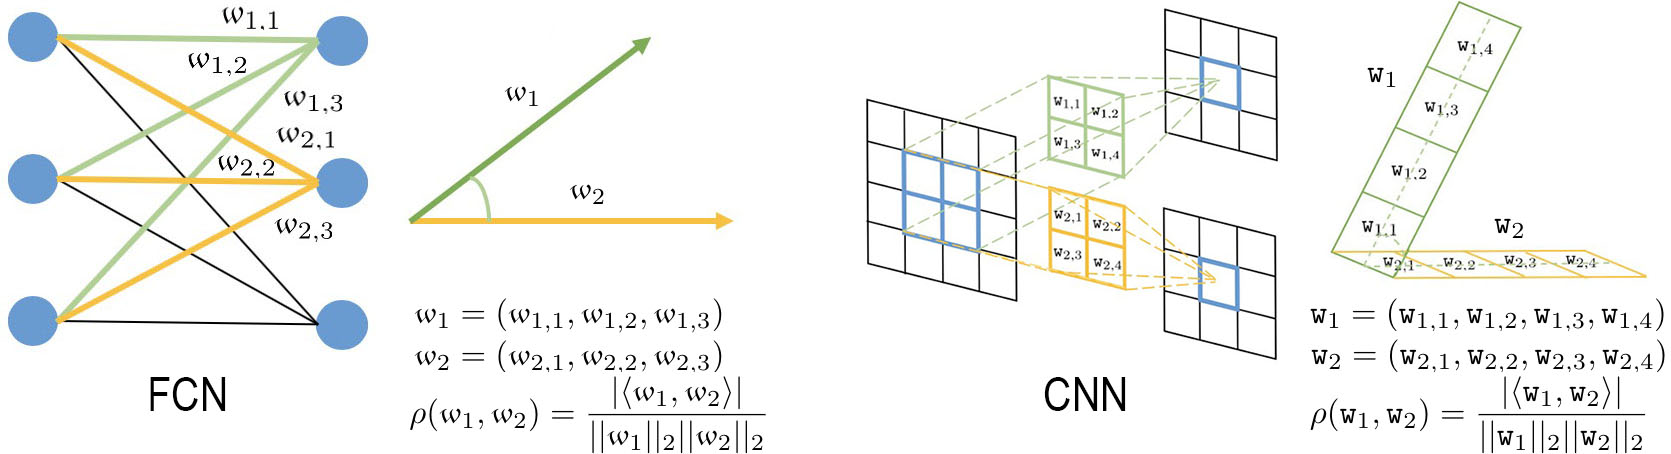
\includegraphics[width=1
\textwidth]{images/PAC-Bayes/figure3.jpg}
\centering
%\vspace{-2mm}
\caption{\textbf{(FCN)} The weight correlation of any two neurons is the cosine similarity of the associated weight vectors. \textbf{(CNN)} The weight correlation of any two filters is the cosine similarity of the reshaped filter matrices.}    
\vspace{-4mm}
\label{fig:definitions}
\end{figure}

Considering the above $\rho(w_l)$, \cite{jin2020does} introduces a correlation matrix $\Sigma_{\rho(w_l)} \in \mathbb{R}^{N_l \times N_l}$, with diagonal elements being $1$, and off-diagonal ones all $\rho(w_l)$. Then, the posterior corvariance matrix can be represented as $\Sigma_{Q_{w_l}}=\Sigma_{\rho(w_l)} \otimes \sigma_l^2I_{N_{l-1}}$, where $\otimes$ is Kronecker product. Let $g(w)=\sum g(w_l)$ where $g(w_l)$ defined by:
\begin{align}
     g(w_l)
     &= - (N_l-1)N_{l-1} \ln (1-\rho(w_l)) - N_{l-1} \ln(1+(N_l-1)\rho(w_l)).
\end{align}
Then the KL term w.r.t. the $l$-th layer can be given by
\begin{equation}
\label{eq:packl}
\begin{aligned}
\mathrm{KL}(Q || P)_l=\frac{||\theta_l^F-\theta_l^0||_{\mathrm{Fr}}^2}{2\sigma_l^2} + g(w_l),
\end{aligned}
\end{equation}
where $\theta^0$ and $\theta^F$ refer to the value of parameters at initialisation and at the end of training, respectively. Further, when $\sigma_l^2=\sigma^2$ for all $l$, we have $\mathrm{KL}(Q || P) = \sum_{l=1}^L \mathrm{KL}(Q || P)_l$. Given the above derivation, \cite{jin2020does} concludes that the KL term in Equation~\ref{eq:packl} is positively correlated to $g(w_l)$. Naturally, $g(w_l)$ can be considered as a regulariser term in the training function.

The training of a neural network is seen as a process of optimising over an objective function $J(\theta;\textbf{x},y)$. \cite{jin2020does} adds a penalty term $g(w)=\sum_{l} g(w_{l})$, which is a function of $\rho(w)$, to the objective function $J$, and denote the regularised objective function by $\tilde{J}$:
\begin{equation}
    \tilde{J}(\theta;\textbf{x},y) = J(\theta;\textbf{x},y) + \alpha g(w),
\end{equation}
where $\alpha \in [0,\infty)$ is a hyper-parameter that balances the relative contribution of the $g(w_l)$ penalty term. Figure~\ref{fig2} provides an illustrative diagram to show the utility of the regularisation. This regularisation is an effective and computationally efficient tool to enhance generalisation performance in practice~\cite{jin2020does}, which could complement other commonly used regularisers such as weight decay and dropout.  

\begin{figure}[t!]
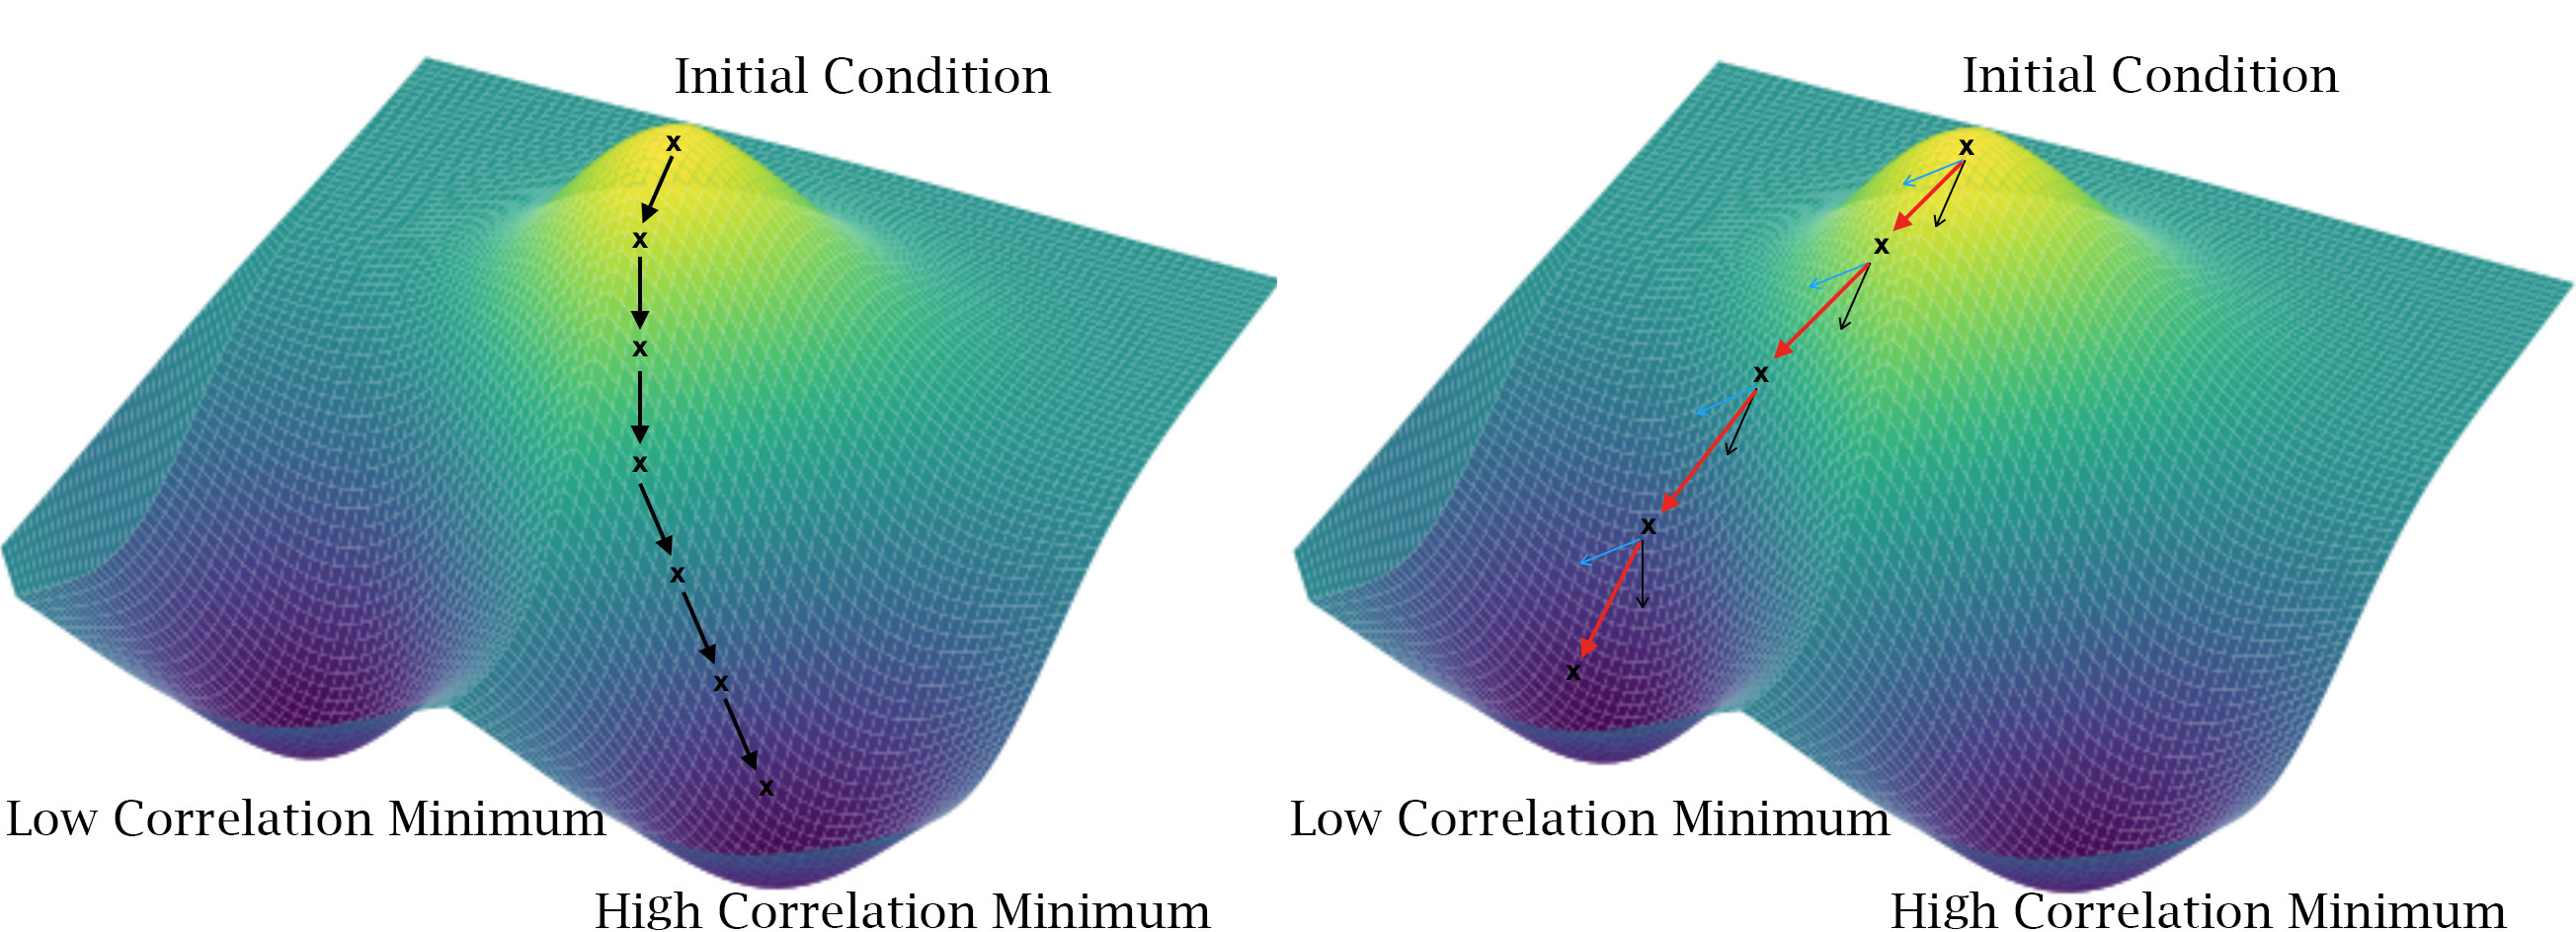
\includegraphics[width=1
\textwidth]{images/PAC-Bayes/figure2_2.jpg}
\centering
%\vspace{-4mm}
\caption{\textbf{Left}: Normal gradient-based optimisers may find a local minimum with high correlation.  \textbf{Right}: Weight correlation regularisation helps the optimiser to find a low correlation minimum, which is more likely to be a global minimum.}    
\vspace{-4mm}
\label{fig2}
\end{figure}
